\documentclass[12pt]{article}
\usepackage{fullpage}
\usepackage{amsmath}
\usepackage{amssymb}
\usepackage{amsthm}
\usepackage{graphicx}
\usepackage{subfigure}
\usepackage{ dsfont }
\usepackage{ mathrsfs }
\usepackage{ mathtools }
\usepackage{hyperref}
%\usepackage{cite}
\usepackage[round]{natbib}
\usepackage{caption}
\usepackage{array}
\usepackage{titling}

%% --------------------- option1 to put Julia code
%% Julia definition (c) 2014 Jubobs
%%
\usepackage{listings}
\usepackage{xcolor}
\definecolor{light-gray}{gray}{0.95}

\lstdefinelanguage{Julia}%
  {morekeywords={abstract,break,case,catch,const,continue,do,else,elseif,%
      end,export,false,for,function,immutable,import,importall,if,in,%
      macro,module,otherwise,quote,return,switch,true,try,type,typealias,%
      using,while,include},%
   sensitive=true,%
%   alsoother={$},%
   morecomment=[l]\#,%
   morecomment=[n]{\#=}{=\#},%
   morestring=[s]{"}{"},%
   morestring=[m]{'}{'},%
}[keywords,comments,strings]%

\lstset{%
    language         = Julia,
    basicstyle       = \ttfamily,
    keywordstyle     = \bfseries\color{blue},
    stringstyle      = \color{magenta},
    commentstyle     = \color{ForestGreen},
    showstringspaces = false,
    backgroundcolor=\color{light-gray},
}

%------------------------------option2 to put Julia code
%%%%% https://gist.github.com/chi-feng/6589066

% \usepackage{inconsolata} % very nice fixed-width font included with texlive-full
% \usepackage[usenames,dvipsnames]{color} % more flexible names for syntax highlighting colors
% \usepackage{listings}

% \lstset{
% basicstyle=\ttfamily,
% columns=fullflexible, % make sure to use fixed-width font, CM typewriter is NOT fixed width
% numbers=left,
% numberstyle=\small\ttfamily\color{Gray},
% stepnumber=1,
% numbersep=10pt,
% numberfirstline=true,
% numberblanklines=true,
% tabsize=4,
% lineskip=-1.5pt,
% extendedchars=true,
% breaklines=true,
% keywordstyle=\color{Blue}\bfseries,
% identifierstyle=, % using emph or index keywords
% commentstyle=\sffamily\color{OliveGreen},
% stringstyle=\color{Maroon},
% showstringspaces=false,
% showtabs=false,
% upquote=false,
% texcl=true % interpet comments as LaTeX
% }

% \lstdefinelanguage{julia}
% {
%   keywordsprefix=\@,
%   morekeywords={
%     exit,whos,edit,load,is,isa,isequal,typeof,tuple,ntuple,uid,hash,finalizer,convert,promote,
%     subtype,typemin,typemax,realmin,realmax,sizeof,eps,promote_type,method_exists,applicable,
%     invoke,dlopen,dlsym,system,error,throw,assert,new,Inf,Nan,pi,im,begin,while,for,in,return,
%     break,continue,macro,quote,let,if,elseif,else,try,catch,end,bitstype,ccall,do,using,module,
%     import,export,importall,baremodule,immutable,local,global,const,Bool,Int,Int8,Int16,Int32,
%     Int64,Uint,Uint8,Uint16,Uint32,Uint64,Float32,Float64,Complex64,Complex128,Any,Nothing,None,
%     function,type,typealias,abstract
%   },
%   sensitive=true,
%   morecomment=[l]{\#},
%   morestring=[b]',
%   morestring=[b]"
% }

\bibliographystyle{mbe} %needs mbe.bst

\newcommand{\falta}[1]{\textcolor{red}{#1}}

\pretitle{%
  \begin{center}
  \LARGE
  \includegraphics[width=6cm,height=2cm]{figures/SNaQ-final-green.pdf}\\[\bigskipamount]
}
\posttitle{\end{center}}

\title{\texttt{PhyloNetworks} Documentation\\
 \large Version 0.0.1}
\author{Claudia Sol\'{i}s-Lemus, C\'{e}cile An\'{e} and John Spaw}
%\date{}

\begin{document}
% http://tex.stackexchange.com/questions/212793/how-can-i-typeset-julia-code-with-the-listings-package
% to put julia code in latex

\maketitle

\section{Introduction}
\texttt{PhyloNetworks} is a \texttt{Julia} package with several functions for
phylogenetic networks, among which we can highlight reading from and
writing in parenthetical format, re-rooting and plotting.
However, the main function in \texttt{PhyloNetworks} is the implementation of
the method \texttt{SNaQ} \citep{Solis-Lemus2015}: a statistical method to
infer a phylogenetic network from input gene trees.

\paragraph{Assumption on the phylogenetic network.} For now, we assume
that the hybridization cycles do not intersect, and these networks are
called \textit{level-1 networks} \citep{Huson2010}. See the appendix
for more details on the definition of phylogenetic networks used here.
This restriction (and others mentioned in the appendix) is enforced
in the optimization, but not in the read/write/plot/root
functions. However, the only rule strictly enforced for all functions
is that a hybrid node cannot have more than two hybrid edges pointing
at it. This is a restriction that we hope to eliminate in the future.

\paragraph{Why Julia?} Julia is a high-level and interactive
programming language (like R or Matlab), but it is also
high-performance (like C). So, it is fast. However, there is a minor
drawback in Julia versions 0.3 (or lower): Julia code is just-in-time
compiled which means that the first time you run a function, it will
take a lot of time because it will compile it. It is important to keep
this in mind as we use Julia, because the next calls for a function
will be much much faster. So, please be patient! Trying out small toy
examples for the first calls of functions is always a good idea.


\section{Setup}
\subsection{Installation of \texttt{Julia}}
To install \texttt{Julia} version 0.3.* (if Julia is already installed, skip
this step): go to\\ \url{http://julialang.org/downloads/}.\\
\texttt{PhyloNetworks} was developed under \texttt{Julia}
version 0.3.5, and has been tested on different versions of 0.3.X.
We have not tested its robustness on \texttt{Julia} version 0.4 or
above, but we will soon. Version 0.4 allows for precompilation, so the
drawback described in the introduction will no longer apply.

\subsection{Installation of \texttt{PhyloNetworks}}
To install the package,
open
\texttt{Julia} and type:
\begin{lstlisting}
Pkg.clone("https://github.com/crsl4/PhyloNetworks.git")
Pkg.build("PhyloNetworks")
\end{lstlisting}

The \texttt{PhyloNetworks} package has the following dependencies, but everything is installed when
\texttt{PhyloNetworks} is added.
\begin{itemize}
\item \texttt{GraphViz} (version 0.0.3)
\item \texttt{NLopt} (version 0.2.0)
\end{itemize}
The version in parenthesis correspond to the ones used when
implementing \texttt{PhyloNetworks}.
To test that you installed correctly the \texttt{PhyloNetworks} package, try the following example:

\subsubsection{Example to test correct \texttt{PhyloNetworks} installation}
Open \texttt{Julia} and type
\begin{lstlisting}
Pkg.test("PhyloNetworks")
\end{lstlisting}
This will take a couple of
minutes as the package needs to compile all the functions. If the
installation was successful, you will see a message at the end:
\textcolor{green}{\textbf{Tests passed}}. Otherwise, an error will be thrown.

\section{Usage of PhyloNetworks}
Before each session, need to type in \texttt{Julia}:

\begin{lstlisting}
using PhyloNetworks
\end{lstlisting}

This will take a couple of minutes as it needs to precompile the
functions.  The first run of a function in \texttt{Julia} will also
compile, so it will be slower than any subsequent runs.

\section{Update of PhyloNetworks}
It is important to regularly update the version of the Julia packages:

\begin{lstlisting}
Pkg.update()
\end{lstlisting}

This will take a couple of minutes as it needs to precompile the
functions in every package. This is particulary important for the
package \texttt{PhyloNetworks} since it is a new package under constant
development.

\paragraph{WARNING:} There is a known bug for Mac users where the \texttt{Pkg.update} function does not update to the latest version. We recommend Mac users to do the following through the terminal:\\
\texttt{
  cd HOME/.julia/v0.3/PhyloNetworks/ \\
  git pull } \\where HOME is replaced by your home directory and v0.3
could be replaced by v0.4 if you have version 0.4 of Julia.

\section{Description of main functions}
Functions in \texttt{Julia} that end with exclamation sign \textbf{!}
are modifying one (or all) of the arguments. The description of the
functions in \texttt{PhyloNetworks} is next:
\begin{itemize}
\item \textbf{readTopology:} Function to read a tree or network from
  parenthetical format. Input can be a string or a name of a text file
  (text file should contain only one line with the tree and end in ;,
  no quotes. To read more than one tree, see \texttt{readInputTrees}
  funcion). This function returns a \texttt{HybridNetwork} object. This
  function allows for many topologies that can be forbidden with the
  restriction described above. That is, this function allows for
  polytomies in tree nodes (tree node with more than two children) and
  internal nodes with only two edges. \
%falta{(and other things not tested yet)}.
\\Usage:
\begin{lstlisting}
net=readTopology(filename);
net=readTopology(string);
\end{lstlisting}
WARNING: it is preferable to end the command with \textbf{;} to avoid
printing to screen some inner details on the network object.


\item \textbf{readTopologyLevel1:} Same as \texttt{readTopology}, but
  this function enforces the restrictions on the network. \texttt{readTopology}
  should be used when you want more variety of topologies, but these
  topologies cannot be used directly as starting point in the
  \texttt{SNaQ} optimization method (which is taken care automatically
  inside the optimization function). This
  function also returns a \texttt{HybridNetwork} object. \\
  Usage:
\begin{lstlisting}
 net=readTopologyLevel1(filename);
 net=readTopologyLevel1(string);
\end{lstlisting}
WARNING: it is preferable to end the command with \textbf{;} to avoid
printing to screen some inner details on the network object.


\item \textbf{tipLabels:} Prints list of taxon names in the \texttt{HybridNetwork}
  object.\\
Usage:
\begin{lstlisting}
tipLabels(net)
\end{lstlisting}

\item \textbf{writeTopology:} Function to write the parenthetical
  format of a \texttt{HybridNetwork} object. It has four options:
\begin{itemize}
\item{\textit{di=true}: to print in a format that Dendroscope can
    read, that is, without the $\gamma$ values (default
  false)}
\item{\textit{outgroup=taxon name}: to root by the outgroup before
    printing (default none). The outgroup has to be a single taxon. We will update to
  allow a clade in the future.}
\item{\textit{names=true}: to print the taxon names in the leaves as opposed to
  the node numbers (default true).}
\end{itemize}
Usage:
\begin{lstlisting}
writeTopology(net)
writeTopology(net,di=true)
\end{lstlisting}

\item \textbf{root!:} Function to root a network at a node or outgroup
  (single taxon). When a node number is used as parameter, you have
  the \textit{resolve} option. If true, a branch with zero length is
  added. The node numbers can be known with the plot function
  described in section \ref{sectPlot}.\\
Usage:
\begin{lstlisting}
root!(net,nodeNumber,resolve)
root!(net,outgroup)
\end{lstlisting}

\item \textbf{deleteLeaf!:} Function to delete a leaf from a
  \texttt{HybridNetwork} object.\\
Usage:
\begin{lstlisting}
deleteLeaf!(net,taxonName)
\end{lstlisting}


\item \textbf{printEdges:} Function to print out the information on
  all the edges in a
  \texttt{HybridNetwork} object. Not all information is useful for the
  user, but information like \textit{edge length} and \textit{gamma}
  are printed.\\
Usage:
\begin{lstlisting}
printEdges(net)
\end{lstlisting}


\item \textbf{printNodes:} Function to print out the information on
  all the nodes in a
  \texttt{HybridNetwork} object. Not all information is useful for the
  user, but information like \textit{node number}
  is printed.\\
Usage:
\begin{lstlisting}
printNodes(net)
\end{lstlisting}

\end{itemize}

\section{\texttt{SNaQ}: estimation of phylogenetic network}

\subsection{Read your data}
\texttt{SNaQ} estimates a phylogenetic network with the statistical
methodology described in \citep{Solis-Lemus2015}. There are two possible
input data:
\begin{itemize}
\item{List of estimated gene trees: Estimated gene trees can be
    obtained from sequence data using RAxML \citep{raxmlv8} or
    MrBayes \citep{Huelsenbeck2001}. Trees need to be in parenthetical
    format. Other formats will be available in future versions of the
    package.}
\item{Table of estimated concordance factors (CF): Estimated CF can be
    obtained from estimated gene trees with BUCKy \cite{Ane2007}.}
\end{itemize}
The methodology also requires a starting topology for the search. This
can be read from parenthetical format.

\noindent Functions to read data into \texttt{Julia}:
\begin{itemize}
\item \textbf{readTrees2CF:} function that read a text file with a
  list of trees in parenthetical format (one tree per line, but it can
  have extra lines like headline that the function will ignore. It
  will assume that any line starting with ``(`` is a tree). The
  function will calculate the observed CF for the corresponding
  4-taxon subsets. There are two possibilities for the 4-taxon subsets: one, the
  list of desired 4-taxon subsets to analyze can be given in a text file
  (\textit{quartetfile name}), and two, if no such file is specified,
  then the user can set a number of 4-taxon subsets (\textit{numQ}) to
  be chosen randomly (\textit{whichQ=:rand})
  from the set of all possible 4-taxon subsets: $n \choose x$ or else all the
  quartets will be considered. \textit{numQ} needs to be
  smaller than the total number of quartets.
  This function will also write by default a text file
  with a table of CF called ``tableCF.txt'', but the name can be
  specified by \textit{filename} and if you do not want to write such table,
  set \textit{writetab=false}. If the quartet file is not specified, then by
  default it will find quartets from the union of all taxa in the tree
  file, but you can choose the set of taxa for the quartets with the
  argument \textit{taxa}.  The function does not need all the arguments,
  see below examples for details.
  \\

  WARNING: This function has not yet been tested with missing
  data. That is, it has been tested in
  examples where all the trees have the same taxa.\\
  Usage:
\begin{lstlisting}
readTrees2CF(treefile, quartetfile, whichQ, numQ,
             writetab, tablename)
readTrees2CF(treefile, whichQ, numQ, taxa, writetab,
             tablename)
\end{lstlisting}

\item \textbf{readTableCF:} Function to read a table of observed
  CF. The table should contain 7 columns as in Table \ref{tableCF}.\\
\begin{table}[h]
\centering
\begin{tabular}{c|c|c|c|c|c|c}
Taxon1 & Taxon2 &Taxon3 & Taxon4 & $CF12|34$ & $CF13|24$ &  $CF14|23$\\
\hline \\
 & & & & & &
\end{tabular}
\caption{Example of column format for the table of CF to be used as
  input data}
\label{tableCF}
\end{table}

Usage:
\begin{lstlisting}
readTableCF(filename);
\end{lstlisting}

Both functions \texttt{readTrees2CF} and \texttt{readTableCF} return a
data structure called \texttt{DataCF} that contains the following
attributes:
\begin{itemize}
\item{quartet: Array with the 4-taxon subsets either read from a table of CF
    or chosen to be analyzed from a list of trees.}
\item{numQuartets: Number of 4-taxon subsets}
\item{tree: Array of \texttt{HybridNetwork} objects that represent the
  list of estimated trees read. If the input data was not a list of
  trees, this attribute will be empty.}
\item{numTrees: Number of trees read.}
\end{itemize}


\item \textbf{readInputTrees:} read a text file with a list of trees
  in parenthetical format (one per line, ignores any line that does
  not start on ``(``) and
  returns a vector of trees.\\
  Usage:
\begin{lstlisting}
readInputTrees(filename)
\end{lstlisting}

\item \textbf{summarizeCFdata:} takes as input a data structure \texttt{DataCF} (from
  previous functions) and provides a few descriptive information. By
  default, it prints the information on the screen, but it can be
  saved to a file. The option \textit{pc} is used only when CF were
  computed from a collection of gene trees: CF for 4-taxon subsets
  that were computed with less than \textit{pc} percentage of the gene
  trees will be listed. The option \textit{pc} should be a number
  between 0 and 1.\\
Usage:
\begin{lstlisting}
summarizeCFdata(d)
summarizeCFdata(d,filename)
summarizeCFdata(d,filename,pc)
\end{lstlisting}

\item \textbf{readStartTop:} read a tree in parenthetical format from
  a text file and updates its branch lenghts with the CF data on
  the data structure \texttt{DataCF}. It is equivalent to run
  readTopologyUpdate first and then updateBL!(net,d)\\
  WARNING: updateBL only works for a tree topology, not proven for a
  network yet.\\  Usage:
\begin{lstlisting}
readStartTop(treefile, d)
\end{lstlisting}

\end{itemize}

\subsubsection{Small example on reading data}
\label{readDataEx}
All the files for this section can be downloaded from the
\textit{examples} folder in github repository. You need to have them
in your working directory.
Suppose you have a file with a list of gene trees called
\textit{treefile.txt} and you want to use all the possible 4-taxon subsets for the
taxa in those trees to calculate the CF:
\begin{lstlisting}
d1=readTrees2CF("treefile.txt")
\end{lstlisting}
If you want to use a random sample of 100 4-taxon subsets:
\begin{lstlisting}
d2=readTrees2CF("treefile.txt",whichQ=:rand,numQ=100)
\end{lstlisting}
On the contrary, if you have already the CF in a file \textit{tableCF.txt}
in the format on Table \ref{tableCF}, you
would read it like:
\begin{lstlisting}
d=readTableCF("tableCF.txt")
\end{lstlisting}
If you have a tree \textit{startTree.tre} in parenthetical format to
use as starting point for the optimization and want to
update the branch lengths according to the CF already read in the data
structure \textit{d}:
\begin{lstlisting}
T=readStartTop("startTree.tre",d);
\end{lstlisting}



\subsection{Estimation method}
The function \texttt{snaq} runs the estimation method described in
\citep{Solis-Lemus2015} and it needs two parameters: starting
topology and a data object \texttt{DataCF}:
\begin{lstlisting}
snaq(startingTopology,data)
\end{lstlisting}
The function has the following options (with default values in parenthesis):
\begin{itemize}
\item \textbf{Nfail} \textit{(100)}: number of proposal failed allowed before
  stopping the optimization
\item \textbf{hmax} \textit{(1)}: maximum number of hybridizations
  allowed
\item \textbf{ftolRel} \textit{(1e-5)}: relative tolerance on the function for the numerical
optimization
\item \textbf{ftolAbs} \textit{(1e-6)}: absolute tolerance on the function for the numerical optimization
\item \textbf{xtolRel} \textit{(1e-3)}: relative tolerance on the parameters for the numerical optimization
\item \textbf{xtolAbs} \textit{(1e-4)}: absolute tolerance on the parameters for the numerical optimization
\item \textbf{verbose} \textit{(false)}: if true, it prints the details of the numerical optimization
\item \textbf{runs} \textit{(10)}: number of independent starting points. The
  first two runs start with the starting topology, and subsequent runs
  modify it by an NNI move. The addition of the initial hybridizations
  (if the starting topology has fewer hybridizations than
  \textit{hmax} are done at random and the seeds are saved)
\item \textbf{outgroup} \textit{(none)}: name of outgroup taxon to root the estimated
network at the end
\item \textbf{filename} \textit{(snaq)}: rootname for the output files: .log, .out, .err
\item \textbf{returnNet} \textit{(true)}: if true, the \texttt{snaq} function
  returns the resulting \texttt{HybridNetwork} object. If false, the
  resulting network is only written in the .out file.
\item \textbf{seed} \textit{(0)}: seed to replicate the
  analyses. This is the main seed from which one seed per run will be
  drawn randomly. To replicate the results for all the runs, simply
  set the same seed. If you want to replicate the results of a given
  run, set \textit{runs=1} and as seed the seed reported in the log
  file for the given run. With default, the clock time is used to
  define the main seed.
\item \textbf{probST} \textit{(0.3)}: probability to use the starting
  topology as the starting point of each run. To improve the
  optimization, it is important that each run starts in a different
  place. At the beginning of every run, a biased coin is thrown so
  that with probability \textit{probST}, the starting topology is not
  changed and with probability \textit{1-probST}, an NNI move is
  performed on the starting topology. If on top the starting topology
  is a network, a second biased coin is flipped with the same
  probability so that with probabiliy \textit{1-probST} we propose
  half the times move origin or and half the times move target.
\end{itemize}

WARNING: the method does not currently have a way to control for the
complexity of the network, so it is important to try to avoid
overparametrizing the model by selecting a very big \texttt{hmax} from
start. It is best to start with \texttt{hmax=1}, and increase
arithmetically trying to keep the estimated network
interpretable. Keep in mind also that the fact that we estimate
\textit{level 1 networks} means that the hybridization cycles cannot
overlap. If the number of taxa is small, and \texttt{hmax} is set very
big, then the method will not be able to place that many
hybridizations.

\subsubsection{Small example on estimating phylogenetic network}
You have $d,T$ from previous example (\ref{readDataEx}), you can
estimate the phylogenetic network by:
\begin{lstlisting}
net=snaq(T,d);
net=snaq(T,d,hmax=2);
\end{lstlisting}
These runs might take a few minutes. The estimated network will be
stored in \texttt{net}, so that the user that write in parenthetical
format, re root or plot:
\begin{lstlisting}
PhyloNetworks.plotPhylonet(net)
\end{lstlisting}
More on the plot function below. There will also be output files
created with information on the estimation procedure.

\subsection{Read .out file}
\begin{itemize}
\item \textbf{readSnaqNetwork:} reads the .out file generated by the
  \texttt{snaq} function and returns a \texttt{HybridNetwork}
  object.\\
Usage:
\begin{lstlisting}
readSnaqNetwork(outfile)
\end{lstlisting}
\end{itemize}

The .log file contains information on the heuristic optimization
such as the seed for each run, the reason why the optimization stopped
(there are different criteria, mostly either there have been too many
failed proposals or the likelihood is not changing anymore), the
number of iterations needed for the algorithm to converge, the value
of the likelihood for the estimated network, and the
number of moves proposed and accepted.

\subsection{Multiple alleles}

The usual settings for SNaQ consider each allele in the gene trees to
be its own tip in the network, however, if there is a known mapping
file of allele names to species, and only the species-level network
wants to be estimated, this can be done with the following functions:
\begin{itemize}
\item{\textbf{mapAllelesCFtable:} This function will read the original
  CF table with allele names, and a mapping file matching allele names
to species names, and return a CF data frame with the allele names
changed to species names. If the option \textit{filename} is defined,
then the new table is also saved as a csv file.
\\Usage:
\begin{lstlisting}
  new_df = mapAllelesCFtable(mappingFile, CFtable);
  new_df = mapAllelesCFtable(mappingFile, CFtable,
           filename="newTable.txt");
\end{lstlisting}
This dataframe should be read also to create a DataCF object:
\begin{lstlisting}
  new_d = readTableCF(new_df);
\end{lstlisting}
The mapping file should have two columns names \textit{alleles} and
\textit{species}. The function will prompt an error if the column
names do not match. It allows for extra columns, and the function will
ignore them.
The estimation will work in the same way:
\begin{lstlisting}
  new_net = snaq(newT,new_d);
\end{lstlisting}
where \textit{newT} should be a starting topology on the species names.
}
\end{itemize}



\subsection{Optimizing branch lengths and inheritance probabilities
  for a given network}
\begin{itemize}
\item \textbf{topologyMaxQPseudolik!:} For a given network, you can
  optimize the branch lengths and inheritance probabilities with the
  pseudolikelihood. Minus the logarithm of the pseudolikelihood value
  for the network will be stored in the attribute: \texttt{net.loglik}
  and it will be printed to screen. The option \texttt{verbose} will
  print the iterations to the screen. The user can also define the
  absolute and relative tolerance with the same options as described
  before for the \texttt{snaq} function. The maximum value allowed for
  branch lengths is 10 (coalescent units).
  \\
  Usage:
  \begin{lstlisting}
    topologyMaxQPseudolik!(net,d)
    topologyMaxQPseudolik!(net,d,verbose=true)
  \end{lstlisting}
  This function is useful to compare the pseudolikelihood of different
  network alternatives, and choose the best one among them.

\item \textbf{topologyQPseudolik!:} For a given network with branch
  lengths and inheritance probabilities, you can compute the
  pseudolikelihood value without optimizing. This function is not
  maximizing, it is simply computing the pseudolikelihood for the
  given branch lenghts and probabilities of inheritance. It is
  advisable though to maximize the pseudolikelihood even when branch
  lengths and probabilities of inheritance are given. This is simply
  because the optimization procedure is quite fast (so it does not
  represent any computational burden) and it will provide a more
  accurate pseudolikelihood value.
  \\
  Usage:
  \begin{lstlisting}
    topologyQPseudolik!(net,d)
    topologyQPseudolik!(net,d,verbose=true)
  \end{lstlisting}
\end{itemize}



\subsection{Debugging: the .err file}
\texttt{SNaQ} is a complex computational algorithm, so despite our
best efforts, there are probably many undetected bugs and errors. The
user can be extremely helpful in fixing this.
After you do any analysis, please check the .err file to check how
many runs failed because of a bug:
\begin{lstlisting}
Total errors: 1 in seeds [4545]
\end{lstlisting}

The seed that caused the error and
the description of the error (which will not necessarily be
informative for the user) will be listed in the .log file.
To help us out to debug \texttt{SNaQ}, please use the same settings
under which you found the error to run the function and the seed in
the .err file associated to the bug:
\begin{lstlisting}
const DEBUG = true
const REDIRECT = true
snaqDebug(T,d,hmax=2,seed=4545);
\end{lstlisting}
This will create two text files: \textit{snaqDebug.log} and
\textit{debug.log}.

You can send them to
\textit{claudia@stat.wisc.edu} with subject \textit{Snaq bug found} or
something similar. I
will not have access to any of your data, the files simply print the
steps I need to retrace the bug and hopefully, fix it.

Errors with the other functions are not straight-forward to detect,
but if you encounter a problem with them, simply type:
\begin{lstlisting}
const DEBUG = true
\end{lstlisting}
and re run the function saving the output to a file and send me that
file.

\section{Phylogenetic Network Visualization}
\label{sectPlot}
This package contains functionality for creating visual plots of
phylogenies generated using the \texttt{SNaQ} estimation method \citep{Solis-Lemus2015}.
The included visualization tools allow the user to plot entire networks with many hybridization events or the underlying tree structure.
Plots created by this package include a dynamic representation of probability of inheritance for hybridization events, which are represented by variation in hybrid edge thickness.
Numerous customization options are available and are described in detail below.

\subsection{Basic Network Plotting}

Plotting with the \texttt{PhyloNetworks} package is simple, being entirely contained in the function \texttt{plotPhylonet}.
Although there are  many optional arguments available for this function, the only \textit{required} input is the network itself.
Networks may be input into \texttt{plotPhylonet} as one of two possible formats, depending on the user's particular preference:
\begin{enumerate}
\item Newick parenthetical format
\item HybridNetwork data type
\end{enumerate}

\noindent Calling this function on a network will generate a .svg image file in the user's working directory
as well as the corresponding .dot file used for rendering. \\

\noindent The .svg file type can be opened and viewed using a number
of different programs including most web browsers (Inkscape, Chrome, Safari, etc.).
If the user wishes to use a different image type, there are a number of options available (two of which we will describe here).
First, the user can access one the many conversion tools that are available on the web. Many of these websites can convert a .svg image into a wide variety of standard image file types.
Another option is to open the corresponding .dot file using GraphViz (which should already be installed) and exporting into the desired format.

\subsection{Customization options}

The \texttt{plotPhylonet} function contains a variety of optional arguments that may be used to tailor the output image to a particular use.
A complete list of optional arguments is given below along with default values and argument descriptions.

\begin{itemize}
\item \textbf{mainTree} \textit{(false)}: When true, only the underlying tree structure is plotted as determined by gammaThreshold. Otherwise, the entire network is shown.

\item \textbf{imageName} \textit{(netImage)}: Name for the output plot.

\item \textbf{gammaThreshold} \textit{(0.5)}: Set's the lowest gamma value to be included when plotting the underlying tree structure.

\item \textbf{width} \textit{(6.0)}: Sets the width of the image in inches.

\item \textbf{height} \textit{(8.0)}: Sets the height of the image in inches.

\item \textbf{vert} \textit{(true)}: When true, the hierarchy of the plot is directed vertically with the root node being place on top and the leaf nodes on bottom.
  Otherwise, the hierarchy is directed horizontally with the root on the left and leaf nodes on the right.

\item \textbf{internalLabels} \textit{(false)}: When true, node labels are included on all internal nodes. Otherwise, they are only included for leaf nodes.

\item \textbf{fontSize} \textit{(16.0)}: Sets the font size for node and edge labels in points.

\item \textbf{layoutStyle} \textit{(``dot")}: Chooses the layout engine used by GraphViz for determining node and edge placement (more details can be found at \url{http://www.graphviz.org/Home.php}.	        							 	     Alternative options include ``neato", ``fdp", ``sfdp", ``circo", and ``twopi".

\item \textbf{hybridColor} \textit{(``green4")}: Sets the color for hybrid edges. Complete list of color options can be found at \url{http://www.graphviz.org/doc/info/colors.html}

\item \textbf{forcedLeaf} \textit{(true)}: When true, leaf nodes are placed on the same level, ranked at the bottom of the network.

\item \textbf{unrooted} \textit{(false)}: Plots an unrooted network or tree using the \textit{neato} engine.

\item \textbf{nodeSeparation} \textit{(0.8)}: Sets the minimum distance between any two nodes in inches.

\item \textbf{edgeStyle} \textit{("line")}: Chooses the edge style used in the plot. Additional options include ``ortho", ``curved", ``composite", "spline", and "false".

\item \textbf{labelAngle} \textit{(180.0)}: Sets the angle of leaf label placement relative to its parent edge.

\item \textbf{labelDistance} \textit{(3.0)}: Sets the distance of leaf label placement relative to its corresponding node.

\item \textbf{includeGamma} \textit{(false)}: When true, gamma labels are included on hybrid edges.

\item \textbf{IncludeLength} \textit{(false)}: When true, length labels are included on all edges.

\end{itemize}


\subsection{Visualization Examples}

This section will provide explicit examples for using the visualization tools provided in the PhyloNetworks package.
Plotting examples will use $(((((1,2))\#H1,(\#H1,(3,4))),5),6);$ as an example network. \\

\noindent \textbf{Example 1:} As previously mentioned, the most simple way to use the included visualization tools is to call the \texttt{plotPhylonet()} function with the network as an argument.
Using our example network, this would be done by typing in
\texttt{Julia}
\begin{lstlisting}
PhyloNetworks.plotPhylonet("(((((1,2))#H1,(#H1,(3,4))),5),6);")
\end{lstlisting}

This will result in the image below being saved in your working directory as \texttt{netImage.svg}.
The file name can be pre-specified when calling \texttt{plotPhylonet} by including the argument \texttt{imageName="newfilename"}, which saves the plot as \texttt{newfilename.svg}.

\begin{figure}[htbp]
  \begin{center}
    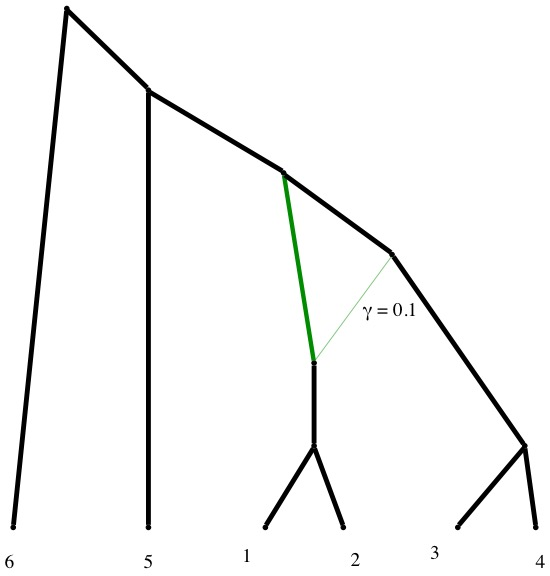
\includegraphics[scale=0.5]{figures/basicplot.pdf} \quad
    \caption{Basic plot using the \texttt{plotPhylonet} function. Note that if the gamma value for a hybrid edge is not explicitly defined, it will assume a default value of $0.1$.}
    \label{BasicPlot}
  \end{center}
\end{figure}

\noindent Calling additional customization options is as simple as including additional arguments separated by a comma.
The user can combine any number of the available arguments to tailor a plot to their particular example.
Given below are a few examples that exhibit the different visualization options available. \\

\noindent \textbf{Example 2:} For the sake of tidiness, we define the network  as its own variable, \texttt{net}.
In addition, we include the arguments \texttt{vert = false}, which plots the hierarchy horizontally,
\texttt{mainTree=true}, which only plots the underlying tree structure, and
\texttt{fontSize = 20.0}, which increases the label font size from 16.0 to 18.0. \\

\begin{lstlisting}
net = "(((((1,2))#H1,(#H1,(3,4))),5),6);"
PhyloNetworks.plotPhylonet(net, vert = false,
                           mainTree = true, fontSize = 20.0)
\end{lstlisting}

\begin{figure}[htbp]
  \begin{center}
    \includegraphics[scale=0.5]{figures/plot2.pdf} \quad
    \caption{Plot of the underlying tree structure, oriented horizontally, with a changed font size.}
    \label{BasicPlot}
  \end{center}
\end{figure}

% INCLUDE UNROOTED EXAMPLE

\subsection{Style Notes}
Although there are default argument values given by \texttt{plotPhylonet}, they do not always result in the ideal plot for a particular example.
Many of the included arguments were included for the purpose of the user being able to adjust certain layout parameters to best fit their own network.
In particular, there is sometimes difficulty in neatly placing and orienting leaf labels and gamma labels.
This is especially noticeable as the number of leaf nodes becomes large or if the the names associated with leaf nodes are long.
We have included some tips for fixing common issues below.

\begin{itemize}
\item To avoid edges overlapping gamma labels, include the argument \texttt{edgeStyle = true}. This will allow the layout engine to include curved splines, which will avoid overlaps.
\item If leaf names are long, include the \texttt{vert = false} argument to set horizontal hierarchy.
\item Label overlap can also be finely altered by changing the \texttt{labelDistance} and \texttt{labelAngle} arguments.
\item Issues between in text readability can be fixed by adjusting the \texttt{fontSize}, \texttt{height}, or \texttt{width}.
\item Although the arguments \texttt{layoutStyle} and \texttt{edgeStyle} have been included,
  some of options available are not guaranteed to be ideal for certain network plots.
\end{itemize}

When plotting, a known issue can occur if Julia and GraphViz are not
linked. To test the GraphViz installation, see the following section:

\subsubsection{Example to test correct \texttt{GraphViz} installation}

The \texttt{GraphViz} package installs the program
\texttt{GraphViz}. To verify that the link between \texttt{Julia} and
\texttt{GraphViz} is working properly. Everything should be done
automatically, but it is worth testing.  Open \texttt{Julia} and type
\begin{lstlisting}
s=open("graph.dot","w")
write(s,"graph {
		a -- b;
		a -- c;
		b -- d;
		b -- e;
		c -- f;
		c -- g;
        f -- h;
        f -- i;
	}")
close(s)
PhyloNetworks.generalExport("graph.dot")
\end{lstlisting}
This will turn
\texttt{graph.dot} into a file called \texttt{genImage.svg} in the
working directory.

\noindent If this worked correctly, the console should display a series of prompts indicating its completion.
A file called \texttt{scratchimage.svg} should be located in your working directory.

\begin{center}
  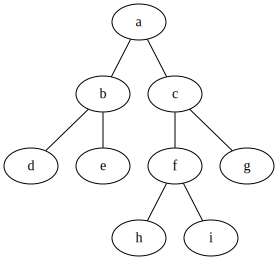
\includegraphics[width=3.0in]{figures/genImage.eps}
\end{center}
Plot of the underlying tree structure, oriented horizontally, with a changed font size.


WARNING: There is a known bug in the \texttt{plotPhylonet} function,
see the issue in the \texttt{PhyloNetworks} Github repository for details.
The error can be sometimes fixed by changing the position of the root
with the \texttt{root} function.

\bibliography{/Users/Clauberry/Documents/phylo/bibtex/Networks-prelim.bib}

\appendix
\section{Definition of Phylogenetic Network}

For the present work, we will use the following definition (but refer
to \citet{Huson2010} for other types of evolutionary networks).
A \textit{rooted phylogenetic network} for a set of taxa $X$ is a
connected directed acyclic graph with vertices $V=V_L \cup V_H \cup
V_T$, edges $E=E_H \cup E_T$ and a bijective leaf-labeling function
$f:V_L \rightarrow X$ with the following characteristics:
\begin{itemize}
\item The root $r$ has $\mathrm{indegree}(r)=0$ and $\mathrm{outdegree}(r)=2$.
\item{For any $v \in V_L$ (leaf), $indegree(v)=1$ and
    $outdegree(v)=0$.}
\item{For any $v \in V_T$ (tree node), $indegree(v)=1$ and $outdegree(v)=2$.}
\item{For any $v \in V_H$ (hybrid node), $indegree(v)=2$ and $outdegree(v)=1$.}
\item{A tree edge $e \in E_T$ is an edge whose child is a tree node.}
\item{A hybrid edge $e \in E_H$ is an edge whose child is a hybrid node.}
\end{itemize}
Thus, we are not allowing internal nodes with only two edges, nor
polytomies. We also do not allow a leaf to be hybrid node, and only 2
hybrid edges per hybrid node.

We also assume that the hybridization cycles do not intersect, and
these networks are called \textit{level-1 networks} \citep{Huson2010},
which have been shown to be identifiable
\citep{Pardi2015,Solis-Lemus2015}.  These restrictions are enforced in
the optimization, but not in the read/write/plot/root
functions. However, the only rule strictly enforced for all functions
is that a hybrid node cannot have more than two hybrid edges pointing
at it. This is a restriction that we hope to eliminate in the future.




\end{document}
